% Created 2016-08-17 Wed 14:38
\documentclass[tikz]{standalone}

\usepackage[utf8]{inputenc}
\usepackage[T1]{fontenc}
\usepackage{helvet}
\usepackage{../../templates/msc}

\renewcommand{\familydefault}{\sfdefault}

\tikzset{
every picture/.style={
line width=1pt
}}

\usepackage{tikz}
\author{Holger Karl}
\date{\today}
\title{}

\usetikzlibrary{decorations.pathreplacing}

\begin{document}

    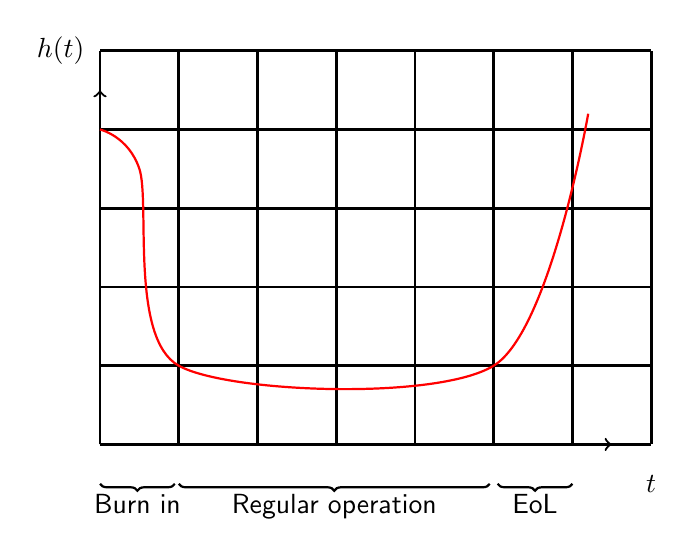
\begin{tikzpicture}
      \draw (0,0) grid (7, 5);
      \draw [thick, ->] (0,0) -- (6.5, 0); 
      \draw [thick, ->] (0,0) -- (0, 4.5); 
      \node at (7, -0.5) {$t$}; 
      \node at (-0.5, 5) {$h(t)$}; 
      % \draw [thick](0,4) -- (1, 1) -- (5, 1) -- (6,4); 
      \draw [thick, red] plot  [smooth ] coordinates {(0,4) (0.5, 3.5)
        (1, 1) (5,
        1)  (6.2,4.2)}; 
      \draw [thick, decorate, decoration={brace}] 
      (0.95, -0.5) -- (0, -0.5) node
      [below,midway] {Burn in};
      \draw [thick, decorate, decoration={brace}] (6, -0.5) -- (5.05, -0.5) node
      [below,midway] {EoL};
      \draw [thick, decorate, decoration={brace}] (4.95, -0.5) -- (1, -0.5) node
      [below,midway] {Regular operation};
    \end{tikzpicture}

\end{document}